% BHU PYQ -- Professional Exam Template
\documentclass[11pt,a4paper]{article}

\usepackage[a4paper,top=2.5cm,bottom=2.5cm,left=2.8cm,right=2.8cm,headheight=14pt]{geometry}
\usepackage{amsmath,amssymb}
\usepackage[T1]{fontenc}
\usepackage[utf8]{inputenc}
\usepackage{lmodern}
\usepackage{microtype}
\usepackage{fancyhdr}
\usepackage{enumitem}
\usepackage{hyperref}
\usepackage{lastpage}
\usepackage{parskip}
\usepackage{tikz}
\usetikzlibrary{arrows.meta,shapes,positioning}

\hypersetup{colorlinks=true,urlcolor=black,linkcolor=black,
  pdftitle={B.Sc. (Hons.) Zoology Sem-V ZOB-503 -- BHU PYQ}}

\pagestyle{fancy}
\fancyhf{}
\renewcommand{\headrulewidth}{0.4pt}
\renewcommand{\footrulewidth}{0.4pt}
\fancyhead[L]{\small   \textit{Banaras Hindu University}}
\fancyhead[R]{\small   \textit{Zoology Paper: ZOB-503}}
\fancyfoot[C]{\small Page  \thepage\ of \pageref{LastPage}}


\newlist{parts}{enumerate}{2}
\setlist[parts,1]{label=(\alph*),leftmargin=*,itemsep=4pt,topsep=3pt}
\setlist[parts,2]{label=(\roman*),leftmargin=*,itemsep=2pt,topsep=2pt}

\newcommand{\pts}[1]{\hfill   \textit{[#1]}}


\begin{document}


\begin{center}
  {\large\bfseries BANARAS HINDU UNIVERSITY}\\[2pt]
  {
\normalsize B.Sc. (Hons.) Semester V Examination, 2022-23}\\[6pt]
  \rule{0.8\linewidth}{0.5pt}\\[6pt]
  {\large\bfseries Zoology}\\[4pt]
  {\large\bfseries Paper: ZOB-503 --- Biochemistry and Molecular Biology}\\[4pt]
  {
\normalsize Time: Three hours \hfill Full Marks: 70}
\end{center}

\rule{\linewidth}{0.4pt}

\smallskip



\noindent   \textit{Note: Answer six questions including Question No. 1 which is compulsory. The figures in the right-hand margin indicate marks.}

\bigskip




\noindent   \textbf{Question 1.} Answer the following parts:

\begin{parts}
  \item State whether the following statements are True or False. Give brief justification for your answer:\pts{$6  \times 2 = 12$}
  
\begin{parts}
    \item SD-sequences help in transcription.
    \item CPSF facilitates initiation of end replication of DNA.
    \item $\alpha$-helix of a protein is stabilized mainly by intrachain disulphide bonds.
    \item Artificially imposed electrochemical gradient can help in ATP synthesis   \textit{in vitro} in absence of succinate and oxygen.
    \item Regulatory enzymes kinetics show a hyperbola curve.
    \item pI of an acidic amino acid is determined by $ \text{pI} = ( \text{pK}_1 +  \text{pK}_2 +  \text{pK}_{ \text{R}})/3$.
  \end{parts}
  
  \item Define the following:\pts{$3  \times 1 = 3$}
  
\begin{parts}
    \item Protein motif
    \item Glycosaminoglycans
    \item Transition state
  \end{parts}

  \item Write the chemical structures of the following:\pts{$2  \times 2.5 = 5$}
  
\begin{parts}
    \item Cholesterol
    
    
\begin{center}
    
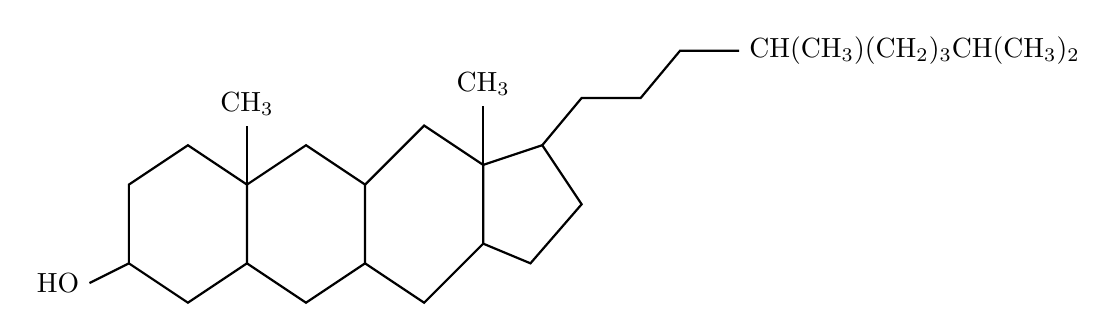
\begin{tikzpicture}[scale=0.5, >=Stealth]
      % Ring A
      \draw[thick] (0,2) -- (1.5,3) -- (3,2) -- (3,0) -- (1.5,-1) -- (0,0) -- cycle;
      
ode at (1.5,1) {A};
      \draw[thick] (0,0) -- (-1,-0.5) node[left] {HO};
      
      % Ring B
      \draw[thick] (3,2) -- (4.5,3) -- (6,2) -- (6,0) -- (4.5,-1) -- (3,0);
      
ode at (4.5,1) {B};
      
      % Ring C
      \draw[thick] (6,2) -- (7.5,3.5) -- (9,2.5) -- (9,0.5) -- (7.5,-1) -- (6,0);
      
ode at (7.5,1.2) {C};
      
      % Ring D
      \draw[thick] (9,2.5) -- (10.5,3) -- (11.5,1.5) -- (10.2,0) -- (9,0.5);
      
ode at (9.9,1.3) {D};
      
      % Methyl groups
      \draw[thick] (3,2) -- (3,3.5) node[above] {CH$_3$};
      \draw[thick] (9,2.5) -- (9,4.0) node[above] {CH$_3$};
      
      % Side chain
      \draw[thick] (10.5,3) -- (11.5,4.2) -- (13,4.2) -- (14,5.4) -- (15.5,5.4) node[right] {CH(CH$_3$)(CH$_2$)$_3$CH(CH$_3$)$_2$};
    \end{tikzpicture}
    \end{center}

    \item Chitin
  \end{parts}
\end{parts}

\medskip


\noindent   \textbf{Question 2.} Discuss the following:

\begin{parts}
  \item Write one cycle of sequence of reactions of a peptide with the Edman's reagent.\pts{5}
  \item Describe the roles of RNA-bound and RNA-free protein complexes in spliceosome mediated splicing.\pts{5}
\end{parts}

\medskip


\noindent   \textbf{Question 3.} Answer the following:

\begin{parts}
  \item Explain the primary level structural constraints of protein folding and the mechanism by which a protein undergoes the folding process.\pts{4}
  \item With the help of at least two examples, justify the statement, ``Quaternary structure provides functional diversity to the protein''.\pts{6}
\end{parts}

\medskip


\noindent   \textbf{Question 4.} Differentiate between the following:\pts{$2  \times 5 = 10$}

\begin{parts}
  \item Uncompetitive and Non-Competitive enzyme inhibition.
  \item DNA-polymerase-$\gamma$ and DNA-polymerase-$\delta$.
\end{parts}

\pagebreak

\medskip


\noindent   \textbf{Question 5.} Answer the following:

\begin{parts}
  \item Illustrate the organization of the pyruvate dehydrogenase complex and its functions.\pts{5}
  \item Illustrate the process of initiation of translation in eukaryotes.\pts{5}
\end{parts}

\medskip


\noindent   \textbf{Question 6.} Answer the following:

\begin{parts}
  \item Indicating all possible details, illustrate the chemiosmotic theory of oxidative phosphorylation.\pts{5}
  
  
\begin{center}
  
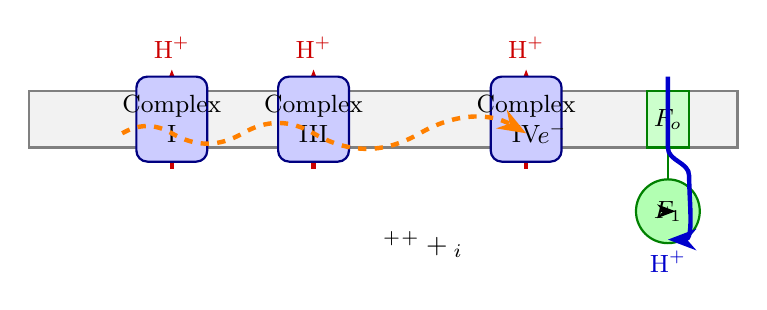
\begin{tikzpicture}[scale=0.9, >=Stealth, every node/.style={font=\small}]
    % Membranes (IMM)
    \draw[fill=gray!10, draw=gray, thick] (-5, 1.5) rectangle (5, 2.3);
    
ode[left] at (-5, 1.9) {   \textbf{IMM}};
    
    % Compartments
    
ode[above] at (0, 2.5) {   \textbf{Intermembrane Space (High $ \text{H}^+$)}};
    
ode[below] at (0, 0.5) {   \textbf{Mitochondrial Matrix (Low $ \text{H}^+$)}};
    
    % Proton pump arrows
    \draw[->, ultra thick, red!80!black] (-3.5, 1.2) -- (-3.5, 2.6) node[above] {$ \text{H}^+$};
    \draw[->, ultra thick, red!80!black] (-1.5, 1.2) -- (-1.5, 2.6) node[above] {$ \text{H}^+$};
    \draw[->, ultra thick, red!80!black] (1.5, 1.2) -- (1.5, 2.6) node[above] {$ \text{H}^+$};
    
    % Complexes
    \draw[fill=blue!20, draw=blue!50!black, rounded corners, thick] (-4, 1.3) rectangle (-3, 2.5) node[pos=0.5, align=center] {Complex\\I};
    \draw[fill=blue!20, draw=blue!50!black, rounded corners, thick] (-2, 1.3) rectangle (-1, 2.5) node[pos=0.5, align=center] {Complex\\III};
    \draw[fill=blue!20, draw=blue!50!black, rounded corners, thick] (1, 1.3) rectangle (2, 2.5) node[pos=0.5, align=center] {Complex\\IV};
    
    % Electron flow
    \draw[->, dashed, ultra thick, orange] (-4.2, 1.7) to[out=30,in=150] (-3.5, 1.7) to[out=-30,in=210] (-2.5, 1.7) to[out=30,in=150] (-1.5, 1.7) to[out=-30,in=210] (0, 1.7) to[out=30,in=150] (1.5, 1.7) node[right, black] {$e^-$};
    
    % ATP Synthase
    \draw[fill=green!20, draw=green!50!black, thick] (3.2, 1.5) rectangle (3.8, 2.3) node[pos=0.5] {$F_o$};
    \draw[fill=green!20, draw=green!50!black, thick] (3.5, 1.5) -- (3.5, 0.9);
    \draw[fill=green!30, draw=green!50!black, circle, thick] (3.5, 0.6) circle (0.45) node {$F_1$};
    
    % Proton flow
    \draw[->, ultra thick, blue!80!black] (3.5, 2.5) -- (3.5, 1.5) to[out=-90, in=90] (3.8, 1.1) to[out=-90, in=0] (3.5, 0.2) node[below] {$ \text{H}^+$};
    
    % Reaction
    
ode[left] at (2.8, 0.6) {$ \text{ADP} +  \text{P}_i$};
    \draw[->, thick] (2.8, 0.6) -- (3.0, 0.6);
    
ode[right] at (4.0, 0.6) {$ \text{ATP}$};
  \end{tikzpicture}
  \end{center}

  \item Describe initiation of replication in eukaryotes with a suitable diagram.\pts{5}
  
  
\begin{center}
  
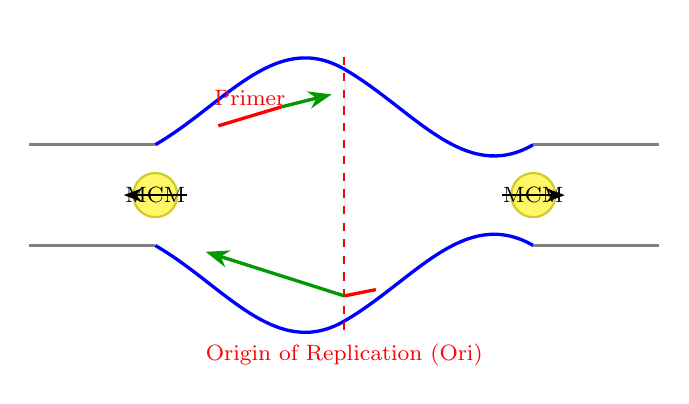
\begin{tikzpicture}[scale=0.8, >=Stealth, every node/.style={font=\footnotesize}]
    % Parental DNA strands
    \draw[very thick, gray] (-5, 0.8) to[out=0, in=180] (-3, 0.8);
    \draw[very thick, gray] (-5, -0.8) to[out=0, in=180] (-3, -0.8);
    
    % Replication bubble
    \draw[very thick, blue] (-3, 0.8) to[out=30, in=150] (0, 2) to[out=-30, in=210] (3, 0.8);
    \draw[very thick, blue] (-3, -0.8) to[out=-30, in=-150] (0, -2) to[out=30, in=-210] (3, -0.8);
    
    \draw[very thick, gray] (3, 0.8) -- (5, 0.8);
    \draw[very thick, gray] (3, -0.8) -- (5, -0.8);
    
    % Origin of replication
    \draw[dashed, red, thick] (0, 2.2) -- (0, -2.2) node[below] {Origin of Replication (Ori)};
    
    % MCM Helicase
    \draw[fill=yellow!60, draw=yellow!80!black, thick] (-3, 0) circle (0.35) node {MCM};
    \draw[fill=yellow!60, draw=yellow!80!black, thick] (3, 0) circle (0.35) node {MCM};
    
    % Direction of unwinding
    \draw[->, thick] (-2.5, 0) -- (-3.5, 0);
    \draw[->, thick] (2.5, 0) -- (3.5, 0);
    
    % RNA Primers and New Strands
    \draw[red, very thick] (-1, 1.4) -- (-2, 1.1) node[midway, above] {Primer};
    \draw[green!60!black, ->, very thick] (-1, 1.4) -- (-0.2, 1.6);
    
    \draw[red, very thick] (0.5, -1.5) -- (0, -1.6);
    \draw[green!60!black, ->, very thick] (0, -1.6) -- (-2.2, -0.9);
  \end{tikzpicture}
  \end{center}
\end{parts}

\medskip


\noindent   \textbf{Question 7.} Answer the following:

\begin{parts}
  \item Write the chemical reactions representing oxidative decarboxylation during Krebs cycle.\pts{5}
  \item Represent the transcription initiation complex on Promoter Type-II.\pts{5}
\end{parts}

\medskip


\noindent   \textbf{Question 8.} Explain the following:\pts{$4 + 3 + 3 = 10$}

\begin{parts}
  \item LB plot helps in better determination of the kinetics parameters of an enzyme.
  
  
\begin{center}
  
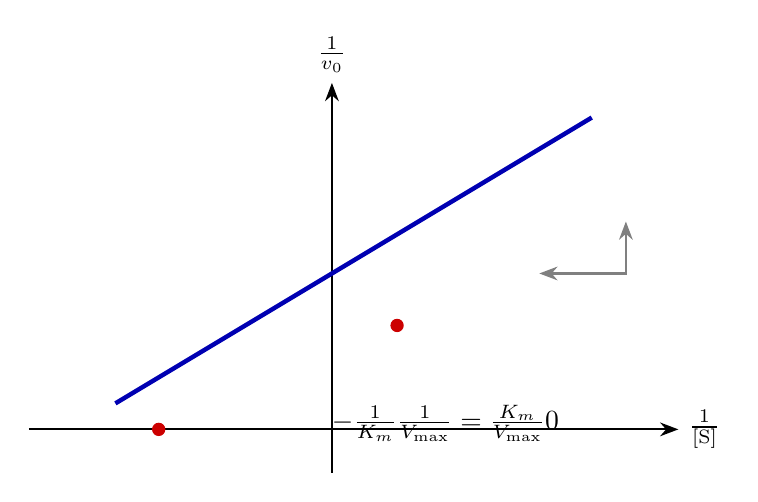
\begin{tikzpicture}[scale=1.1, >=Stealth]
    % Axes
    \draw[->, thick] (-3.5,0) -- (4,0) node[right] {$\frac{1}{[ \text{S}]}$};
    \draw[->, thick] (0,-0.5) -- (0,4) node[above] {$\frac{1}{v_0}$};
    
    % Plot line
    \draw[ultra thick, blue!70!black] (-2.5, 0.3) -- (3, 3.6);
    
    % Important points
    \filldraw[red!80!black] (-2.0,0) circle (2pt);
    
ode[below left, red!80!black] at (-2.0,0) {$-\frac{1}{K_m}$};
    
    \filldraw[red!80!black] (0,1.2) circle (2pt);
    
ode[above right, red!80!black] at (0,1.2) {$\frac{1}{V_{\max}}$};
    
    % Slope indicator
    \draw[<->, thick, gray] (1, 1.8) -- (2, 1.8) -- (2, 2.4);
    
ode[right] at (2, 2.1) {$ \text{Slope} = \frac{K_m}{V_{\max}}$};
    
    
ode[below right] at (0,0) {$0$};
  \end{tikzpicture}
  \end{center}

  \item Animal cells have stored glycogen rather than starch.
  \item HDL are known as ``good cholesterol''.
\end{parts}

\vfill
\rule{\linewidth}{0.4pt}

\begin{center}\small
\href{https://bhu-exam.vercel.app/}{Click Here}\\[4pt]\href{https://me-aryan.vercel.app/}{Click Here}\\[4pt]\href{https://quashan-me.vercel.app/}{Click Here}
\end{center}

\end{document}
